\documentclass[english,,man]{apa6}
\usepackage{lmodern}
\usepackage{amssymb,amsmath}
\usepackage{ifxetex,ifluatex}
\usepackage{fixltx2e} % provides \textsubscript
\ifnum 0\ifxetex 1\fi\ifluatex 1\fi=0 % if pdftex
  \usepackage[T1]{fontenc}
  \usepackage[utf8]{inputenc}
\else % if luatex or xelatex
  \ifxetex
    \usepackage{mathspec}
  \else
    \usepackage{fontspec}
  \fi
  \defaultfontfeatures{Ligatures=TeX,Scale=MatchLowercase}
\fi
% use upquote if available, for straight quotes in verbatim environments
\IfFileExists{upquote.sty}{\usepackage{upquote}}{}
% use microtype if available
\IfFileExists{microtype.sty}{%
\usepackage{microtype}
\UseMicrotypeSet[protrusion]{basicmath} % disable protrusion for tt fonts
}{}
\usepackage{hyperref}
\hypersetup{unicode=true,
            pdftitle={Conceptual Hierarchy in Child-Directed Speech: Implicit Cues are More Reliable},
            pdfkeywords={Conceptual learning, child-directed speech, language and cognition},
            pdfborder={0 0 0},
            breaklinks=true}
\urlstyle{same}  % don't use monospace font for urls
\ifnum 0\ifxetex 1\fi\ifluatex 1\fi=0 % if pdftex
  \usepackage[shorthands=off,main=english]{babel}
\else
  \usepackage{polyglossia}
  \setmainlanguage[]{english}
\fi
\usepackage{graphicx,grffile}
\makeatletter
\def\maxwidth{\ifdim\Gin@nat@width>\linewidth\linewidth\else\Gin@nat@width\fi}
\def\maxheight{\ifdim\Gin@nat@height>\textheight\textheight\else\Gin@nat@height\fi}
\makeatother
% Scale images if necessary, so that they will not overflow the page
% margins by default, and it is still possible to overwrite the defaults
% using explicit options in \includegraphics[width, height, ...]{}
\setkeys{Gin}{width=\maxwidth,height=\maxheight,keepaspectratio}
\IfFileExists{parskip.sty}{%
\usepackage{parskip}
}{% else
\setlength{\parindent}{0pt}
\setlength{\parskip}{6pt plus 2pt minus 1pt}
}
\setlength{\emergencystretch}{3em}  % prevent overfull lines
\providecommand{\tightlist}{%
  \setlength{\itemsep}{0pt}\setlength{\parskip}{0pt}}
\setcounter{secnumdepth}{0}

%%% Use protect on footnotes to avoid problems with footnotes in titles
\let\rmarkdownfootnote\footnote%
\def\footnote{\protect\rmarkdownfootnote}


  \title{Conceptual Hierarchy in Child-Directed Speech: Implicit Cues are More Reliable}
    \author{true \\ true \\ true}
    \date{}
  
% Manuscript styling
\usepackage{upgreek}
\captionsetup{font=singlespacing,justification=justified}

% Table formatting
\usepackage{longtable}
\usepackage{lscape}
% \usepackage[counterclockwise]{rotating}   % Landscape page setup for large tables
\usepackage{multirow}		% Table styling
\usepackage{tabularx}		% Control Column width
\usepackage[flushleft]{threeparttable}	% Allows for three part tables with a specified notes section
\usepackage{threeparttablex}            % Lets threeparttable work with longtable

% Create new environments so endfloat can handle them
% \newenvironment{ltable}
%   {\begin{landscape}\begin{center}\begin{threeparttable}}
%   {\end{threeparttable}\end{center}\end{landscape}}
\newenvironment{lltable}{\begin{landscape}\begin{center}\begin{ThreePartTable}}{\end{ThreePartTable}\end{center}\end{landscape}}

% Enables adjusting longtable caption width to table width
% Solution found at http://golatex.de/longtable-mit-caption-so-breit-wie-die-tabelle-t15767.html
\makeatletter
\newcommand\LastLTentrywidth{1em}
\newlength\longtablewidth
\setlength{\longtablewidth}{1in}
\newcommand{\getlongtablewidth}{\begingroup \ifcsname LT@\roman{LT@tables}\endcsname \global\longtablewidth=0pt \renewcommand{\LT@entry}[2]{\global\advance\longtablewidth by ##2\relax\gdef\LastLTentrywidth{##2}}\@nameuse{LT@\roman{LT@tables}} \fi \endgroup}

% \setlength{\parindent}{0.5in}
% \setlength{\parskip}{0pt plus 0pt minus 0pt}

% \usepackage{etoolbox}
\makeatletter
\patchcmd{\HyOrg@maketitle}
  {\section{\normalfont\normalsize\abstractname}}
  {\section*{\normalfont\normalsize\abstractname}}
  {}{\typeout{Failed to patch abstract.}}
\makeatother
\shorttitle{Conceptual Hierarchy in CDS}
\author{Kyra WILSON\textsuperscript{1}, Michael C. FRANK\textsuperscript{1}, \& Abdellah FOURTASSI\textsuperscript{2}}
\affiliation{
\vspace{0.5cm}
\textsuperscript{1} Department of Psychology, Stanford University\\\textsuperscript{2} Department of Computer Science, Aix-Marseille University}
\authornote{

'All data and analytic code are available at https://github.com/afourtassi/concepts' 

'A preliminary version of this work was presented in the cognitive science society conference and appeared in the  non-archival proceedings as: 

Fourtassi, A., Wilson, K.,  \& Frank, M., C. (2020). Discovering Conceptual Hierarchy Through Explicit and Implicit Cues in Child-Directed Speech. In Proceedings of the 42nd Annual Meeting of the Cognitive Science Society'


Correspondence concerning this article should be addressed to Abdellah FOURTASSI, Postal address. E-mail: abellah.fourtassi@univ-amu.fr}
\keywords{Conceptual learning, child-directed speech, language and cognition}
\DeclareDelayedFloatFlavor{ThreePartTable}{table}
\DeclareDelayedFloatFlavor{lltable}{table}
\DeclareDelayedFloatFlavor*{longtable}{table}
\makeatletter
\renewcommand{\efloat@iwrite}[1]{\immediate\expandafter\protected@write\csname efloat@post#1\endcsname{}}
\makeatother
\usepackage{csquotes}
\usepackage{tipa}
\usepackage[sortcites=false,sorting=none]{biblatex}
\usepackage{tabularx}

\abstract{
In order for children to understand and reason about the world in an adult-like fashion, they need to learn that conceptual categories are organized in a hierarchical fashion (e.g., a dog is also an animal). While children learn from their first-hand observation of the world, social knowledge transmission via language can also play an important role in this learning. Previous studies have documented several cues in parental talk that can help children learn about conceptual hierarchy. However, these studies have used different datasets and methods which has made it difficult to compare the relative usefulness of various linguistic cues to conceptual knowledge and to test whether they scale up to the naturalistic speech. Here, we studies a large-scale corpus of English child-directed speech and used a unified classification-based evaluation method which allowed us to investigate and compare cues that vary in terms of how explicit the information they offer is. We found the more explicit cues to be too sparse or too noisy in child-directed speech, making them unlikely to support robust learning. In contrast, the implicit cues offered a more reliable source of information starting from the linguistic input heard by 3 years and up to 6 years of age. Our work confirms the utility of caregiver talk for conveying conceptual information and supporting the development of early taxonomic knowledge. It provides a first step toward a cognitive model that would combine perceptual- and language-based mechanisms, leading to testable predictions about children's conceptual development.
}

\begin{document}
\maketitle

\hypertarget{introduction}{%
\section{Introduction}\label{introduction}}

A hallmark of human conceptual knowledge is its hierarchical organization. For example, the same entity (e.g., a dog) can be considered in a nested structure as, e.g., a husky, a dog, a mammal, and an animal. Such hierarchical organization is fundamental to human cognition as it allows, among other things, the generalization of knowledge through inference. For example, upon children's learning that all animals eat, they can conclude that giraffes also eat because the category \enquote{giraffe} is \emph{included} in the category \enquote{animal} (e.g., Markman, 1989; Inhelder \& Piaget, 2013; Murphy, 2004; Sloutsky, 2010). The current study asks how this hierarchical knowledge develops? More specifically, we ask whether children can learn conceptual hierarchy from the \emph{language} they hear around them.

Although taxonomic knowledge takes time to mature into an adult-like form (Blaye, Bernard-Peyron, Paour, \& Bonthoux, 2006; Lucariello, Kyratzis, \& Nelson, 1992; Unger, Savic, \& Sloutsky, 2020), researchers have noted that children as young as 3 years old already show signs of hierarchical knowledge in their early lexicon. For example, observational studies have found that children use superordinate words like \enquote{food} and \enquote{animal} (e.g., Fenson et al., 1994; Frank, Braginsky, Yurovsky, \& Marchman, 2021), and they use different labels to refer to the \emph{same} object, shifting their conceptual perspective from one level of abstractness to another (e.g., using the labels \enquote{dog} and \enquote{animal} to refer to a dog) (e.g., Clark, 1997). In more controlled in-lab experiments, preschool children are able, depending on the situation, to interpret the meaning of a novel word (e.g., \enquote{Dax}) either at the basic or at the superordinate level (Callanan, 1989; Markman \& Hutchinson, 1984). Critically, children do not simply extend the meanings of words based only on how objects look, e.g., they do not simply use a novel word (e.g., \enquote{Dax}) to name both a car and a truck (but not, say, a banana) because the shape of a car is more similar to that of a truck than to that of a banana. Under some circumstances, e.g., when using the label to name multiple objects from the target superordinate category, they do prefer taxonomic relations even when a perceptually similar --- but taxonomically unrelated --- alternative is available (Gentner \& Namy, 1999; Liu, Golinkoff, \& Sak, 2001).

How do children begin acquiring the hierarchical structure of semantic knowledge? Early accounts considered this learning to be the consequence of the emergence of a \emph{domain-general} logic of class inclusion --- that one category can be part of a larger one --- which develops through middle childhood (Inhelder \& Piaget, 2013; Winer, 1980). However, and though the logic of classes may represent a mature, adult-like structuring principle of concepts enabling reasoning on both familiar and unfamiliar domains, the above-reviewed evidence suggests that children begin showing, much earlier, the ability for hierarchical reasoning in \emph{specific domains} they are familiar with or interested in (e.g., the domain of food or dinosaurs). This fact suggests that the input they receive in specific domains (whether through perceptual or linguistic means) plays an important role in shaping this organization (See also Chi, Hutchinson, \& Robin, 1989; Carey, 1987; Inagaki \& Hatano, 2002).

Research on the role of children's input in the development of a hierarchical conceptual structure can be summarized into a perceptual/functional-based account and a language-based account (though these accounts are more complementary than mutually exclusive). In the perceptual/functional-based account, children are understood to rely on their first-hand observation of the world, allowing them to form abstract concepts using primarily their ability to pick up on similarities between entities in terms of their perceptual features or functions (Madole \& Oakes, 1999; McClelland \& Rogers, 2003; Quinn \& Eimas, 2000; Sloutsky, 2015, 2010; Smith \& Heise, 1992). Second, using their inductive reasoning skills, they synthesize these concepts into a nested tree structure via performing some sort of hierarchical clustering (Kemp, Perfors, \& Tenenbaum, 2007; Saxe, McClelland, \& Ganguli, 2019; Tenenbaum, Griffiths, \& Kemp, 2006). Finally, children are understood to learn how to attribute multiple labels to the same entity (e.g., dog, mammal, animal), whereby more abstract/broad labels map onto larger regions in the nested tree structure (Xu \& Tenenbaum, 2007).

The current study is, however, best situated within the framework of the language-based account, whereby children are understood to rely, not only on their own perceptual data but \emph{also} on knowledge transmission from other people. Indeed, superordinate concepts (more than basic-level ones) do not necessarily share similar --- sensory accessible --- features. For example, the categories \enquote{animal} and \enquote{plants} are organized for Groote Eylandt Australian aborigines rather into three categories: \enquote{biological}, \enquote{food}, and \enquote{totemic} (Waddy, 1982). Thus, learning conceptual hierarchy requires additional, culture-specific input, primarily via language (Csibra \& Gergely, 2009; Gelman, 2009; Harris, 2012).

Regarding how children may learn conceptual hierarchy from language, observational studies have noted that when parents introduce words at the superordinate level, they typically also provide the basic level term (Callanan, 1985; Shipley, Kuhn, \& Madden, 1983). For example, parents rarely point to an object and say \enquote{this is an animal!} Instead, they usually \emph{anchor} the superordinate word \enquote{animal} at the basic level by saying something along the lines of \enquote{This is a duck; a duck is a kind of animal.} Such an anchoring strategy provides children with a categorization of the same object at different levels, which may help them understand the hierarchical organization.

Also within the language-based account, more recent research, prompted by advances in machine learning (e.g., Mikolov, Sutskever, Chen, Corrado, \& Dean, 2013; Landauer \& Dumais, 1997), found that the statistical distribution of basic-level terms in parental speech can lead to coherent structures at the superordinate level (Fourtassi, Scheinfeld, \& Frank, 2019; Frermann \& Lapata, 2016a; Huebner \& Willits, 2018). For example, though \enquote{fish} and \enquote{bird} do not look very similar, people talk about them in similar linguistic contexts, typically leading to similar distributions in speech. Having a shared pattern of co-occurrence cues taxonomic relations and, in fact, several experimental studies have suggested that it does help to acquire such relations in development (Brown \& Berko, 1960; Ervin, 1961; McNeill, 1963; Sloutsky, Yim, Yao, \& Dennis, 2017).

These linguistic cues can be thought of as ends in a continuum that varies from explicit to implicit. The \enquote{is-a-kind-of} cue is the most explicit cue since both the labels (i.e., the basic and superordinate labels) and their hierarchical relationship are explicitly stated. The \enquote{distributional cue} is the most implicit cue since, on the one hand, the superordinate term is not required and, on the other hand, the hierarchical relationship (that is, the fact that co-occurring basic-level terms are part of a higher-level category) can only be induced.

While the above-reviewed studies have focused on these extremes, one can think of other cues that have an intermediate status on this continuum. We introduce and test two such cues. The first, which we name the \enquote{pragmatic cue,} is when parents hint at the hierarchical relationship between two concepts pragmatically without using an explicit inclusion expression. For example, instead of saying \enquote{a cow is a kind of animal,} parents can say the following: \enquote{Do you want a cow or do you want another animal?} (see Table 1 for more examples). In addition, we also study an \enquote{Affordance-based cue} whereby action affordances provide another -- and perhaps more implicit -- linguistic cue for category membership. For example, food items could be identified as members of a single superordinate category by virtue of their affordance of \enquote{eating} and clothing items by their affordance of \enquote{wearing.} (see Figure \ref{fig:cues}).

\begin{figure}[h]

{\centering 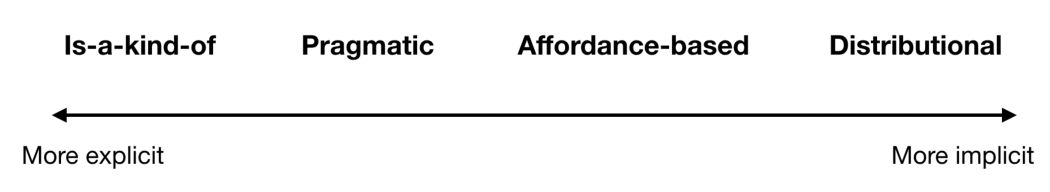
\includegraphics{child_language_journal_files/figure-latex/cues-1} 

}

\caption{\label{fig:cues} The cues to conceptual hierarchy in the linguistic input can be understood as falling on a continuum from most explicit to most implicit.}\label{fig:cues}
\end{figure}

\hypertarget{the-current-study}{%
\subsection{The current study}\label{the-current-study}}

Previous studies examining individual linguistic cues to conceptual hierarchy have varied in terms of both the datasets and methods they used, which has made comparison difficult, thus hindering cumulative scientific progress on this question. On the one hand, implicit cues have generally been studied using large-scale data and have been evaluated based on their ability to provide an accurate similarity space for words. On the other hand, explicit cues have been studied mainly in the context of small-scale experiments and have been tested mainly by counting the frequency of a given linguistic expression (e.g., \enquote{X is a kind of Y}).

In this study, we make a systematic comparison of explicit and implicit cues using similar methods. In particular, we quantify the information provided by each of these cues in Figure 1 using spontaneous -- rather than scripted -- child-directed speech, using language data from naturalistic child-caregiver interactions (CHILDES 2018.1, MacWhinney, 2000; Sanchez et al., 2019). We test information contained in this input data across the entire early lexicon as measured by the MacArthur-Bates Communicative Inventory (CDI) (Fenson et al., 1994). We focus on the hierarchical relations that the basic-level terms in this early lexicon bear on six superordinate labels: Animals, Furniture, Clothes, Food, Toys, and vehicles. This set of superordinate concepts was chosen because it combines all the concepts that had been studied previously and for which CDI data were available. Further, a data-driven approach using CDI words and input from CHILDES (Fourtassi et al., 2019) led to a set of categories made of \enquote{animal}, \enquote{food,} \enquote{clothes,} and a broad category of "artifacts'' which included instances of toys, vehicles, and furniture. Here, we kept the last three categories differentiated as in previous experimental work.

Our research question is to investigate the relative usefulness of each linguistic cue in providing information that children can utilize for learning hierarchical conceptual relationships. To address this question, we proceed as follows. We begin by introducing the child-directed data and the derived linguistic cues for conceptual hierarchy. We then explain the task and evaluation methods that we use to study and compare these cues. Next, we present the results quantifying the role of each of the four cues and their relative informativeness by 3 three years of age as well as their change in development up to 6 years old. Finally, we discuss our findings in light of the literature on early linguistic and conceptual development.

\hypertarget{methods}{%
\section{Methods}\label{methods}}

\hypertarget{data}{%
\subsection{Data}\label{data}}

We constructed a large-scale corpus by aggregating all English-language transcripts from CHILDES (MacWhinney, 2000; Sanchez et al., 2019). We selected all utterances in which the speaker was not tagged as \enquote{Child} or \enquote{Target\_Child.} In other words, we only keep input from adults, excluding language produced by children. In the main analyses, we limit the input to the speech addressed to children up to three years of age as this is the age where early signs of conceptual hierarchy appear according to the above-reviewed developmental literature. That said, we also include results from speech addressed to children up to six years to investigate potential developmental changes in the input. The final corpus contained 1.9 million utterances and 7.9 million words from a collection of 4,939 transcripts across 660 children with an average age of 26.8 months. We decided to study the six following superordinate categories: \enquote{animal}, \enquote{furniture}, \enquote{clothes}, \enquote{food}, \enquote{toys} and \enquote{vehicles.} For each of these categories, we used the corresponding basic-level terms available in the English-language MacArthur-Bates Communicative Inventory (CDI) (Fenson et al., 1994), a parent-report instrument that provides a partial listing and categorization of words produced by children 18--30 months.

\hypertarget{cues-to-conceptual-hierarchy-and-their-feature-vectors}{%
\subsection{Cues to Conceptual Hierarchy and their Feature Vectors}\label{cues-to-conceptual-hierarchy-and-their-feature-vectors}}

As shown in Figure 1, we consider the four linguistic cues to conceptual hierarchy, ranging from most explicit to most implicit: \enquote{is-a-kind-of}, the pragmatic, affordance-based, and distributional cues. To facilitate comparison, we represented all these cues as vectors and we tested how these vectors allow us to classify basic-level terms into superordinate categories. Below we describe in detail how these vectors were constructed. To summarize, for the \enquote{is-a-kind-of} and the pragmatic cues where the hierarchical relation relies on the explicit mention of the superordinate words, the vectors were based on the six superordinate words, and each cell in the vector corresponded to the frequency with which the hierarchical relation was found between the basic-level word at hand and the superordinate word in the current cell (see the illustration in Figure \ref{fig:task}, left). For the affordance-based cue, the vector was constructed in a similar fashion, except that the superordinate terms were replaced with their corresponding affordances (e.g., \enquote{eatable} for food and \enquote{wearable} for clothes) and each of the six cells in the vector corresponded to the frequency with which the basic-level word has been used with the verb that marks the affordance. Finally, the implicit distributional cue does not rely on an explicit category marker. Instead, the feature vector was an \enquote{embedding} in a high dimensional space derived based on the words' shared pattern of co-occurrence.

\hypertarget{is-a-kind-of}{%
\subsubsection{Is-a-kind-of}\label{is-a-kind-of}}

This cue tests the extent to which parents use explicit expressions of class inclusion (Callanan, 1985). For each word at the basic level, \(X\) (e.g., cow),
we construct a feature vector of length 6, where each cell corresponds to one of the 6 superordinate categories under study, \(Y_i\) (e.g., animal or food). The value in cell \(i\) corresponds to the frequency with which \(X\) appears with \(Y_i\) in one of the following expressions: \enquote{\(X\) is a/an \(Y_i\)} or \enquote{\(X\) is a kind/type/sort of \(Y_i\)} (we kept the same expressions used in the previous study).

\hypertarget{pragmatic}{%
\subsubsection{Pragmatic}\label{pragmatic}}

Parents can express conceptual hierarchy between \(X\) and \(Y_i\) without necessarily using an explicit \enquote{is-a-kind-of}-like expression. In many cases, parents can hint at this hierarchy using a wide diversity of linguistic expressions (see Table 1 for examples from our dataset). The precise and exhaustive characterization of these expressions at scale is an open computational challenge. That said, as a first attempt to capture the diversity with which parents hint at conceptual hierarchy in a pragmatic fashion, we relaxed grammatical constraints between \(X\) to \(Y_i\), and we kept only the requirement that \(X\) and \(Y_i\) should co-occur. More concretely, we represent each basic-level term, \(X\), with a feature vector where each cell contains the frequency with which X co-occurs
with the corresponding superordinate term \(Y_i\) (see Figure \ref{fig:task}, left). This co-occurrence is determined using a fixed window of \(k\) utterances. Values of \(k > 1\)
allow us to capture the case where a relationship between \(X\) and \(Y_i\) is established across more than one utterance. For example:

-- Mother: What kind of animal is this?

-- Mother: It's a giraffe!

\begin{table}[!htbp] \centering 

\caption{\label{tab:pragmatic} Examples of utterances from CHILDES where parents hint at hierarchical relations between basic- and superordinate-level terms.}

\begin{tabularx}{\linewidth}{cXXc}
\hline
\textbf{Category} & Utterance & Interlocutors & Corpus\\
\hline

\textbf{Animals} & Do you want a cow or do you want a different animal? & Mother to Max, 30 months & EllisWeismer\\

\textbf{Furniture} & Furniture means sofas and chairs and... & Mother to Naima, 23 months & Providence\\

\textbf{Clothes} & This is another clothes. See it's just like this shirt. & Investigator to Shem, 30 months & Clark\\

\textbf{Food} & She asked Lily what her favorite food was. If Lily says chocolate I am in trouble. & Mother about Lily, 24 months & Providence\\

\textbf{Toys} & You close the book and we'll get a different toy cause I think you're tired of this. & Mother to child, 13 months & Ambrose\\

\textbf{Vehicles} & The only vehicle you cut out so far is the train. & Mother to Warren, 30 months & Manchester\\

\hline
\end{tabularx}

\end{table}

\hypertarget{affordance-based}{%
\subsubsection{Affordance-based}\label{affordance-based}}

The superordinate label is not the only category marker that can cue conceptual hierarchy for a basic level term, especially when this category can also be characterized by its affordance. For example, \enquote{food} can be characterized as the category of things we eat and \enquote{clothes} as things we wear. Thus, children can learn that some concepts (e.g., \enquote{apple} and \enquote{bread}) are parts of a higher-level category (\enquote{things we eat}) by observing how these concepts co-vary with a cue of their common affordance (i.e., the verb \enquote{eat}).

We computed the feature vectors for the affordance-based cue as follows. In a first step, we tried to find a verb that could be used as an affordance marker for an entire category. We used \enquote{eat} for food, \enquote{wear} for clothes, \enquote{play} for toys, and \enquote{ride} for vehicles. The category \enquote{furniture} has no such obvious function verb. We decided to use the verb \enquote{use} because if there were a verb that could fit every member of the category of furniture, it would be that (even though it can also fit things that are not members of the category). For the animal category, we could find no verb that could categorize the instances. In addition to these verbs, we also identified synonymous verbs for each category that could also signify an affordance for the category. However, these verbs were either not found in the corpus (words like \enquote{devour} and \enquote{utilize} are not used in child-directed speech) or they occurred in too many contexts to be useful for categorization (\enquote{have} can be used synonymously with \enquote{eat}, but it has additional meanings that make this not a useable cue). Because of this, only one verb was used for computing the feature vectors for each of the categories.

We detected the affordance-based relationships, syntactically, based on occurrence in a verb-complement structure.\footnote{There are more complex structures that could, in principle, be used by parents. Here we used the simplest.} For example, in the utterance \enquote{the bird eats the berries,} the word \enquote{berries} was categorized as \enquote{eat}-able. For each basic-level term \(X\), we computed a 6-cell-long feature vector where the value in each cell corresponded to the frequency with which\(X_i\) occurs in a verb-complement relationship with the verb/affordance \(Y_i\) at hand.

\hypertarget{distributional-cue}{%
\subsubsection{Distributional cue}\label{distributional-cue}}

Unlike the first three cues, the pure distributional cue is not based on an explicit category marker at the superordinate level. It is based, instead, only on the way basic-level terms are distributed together in speech. According to the distributional hypothesis (Harris, 1957), words that share similar patterns of co-occurrence (or distribution) in speech tend to be semantically close. For example, a child can posit that the words \enquote{apple} and \enquote{banana} must refer to objects that share semantic properties (and likely belong to the same superordinate category) because people around them tend to talk about both words in similar context using similar co-occurring words such as \enquote{eat,} \enquote{kitchen,} \enquote{dessert,} and \enquote{tree.}

Following previous research (Fourtassi et al., 2019), we quantified this cue using a model called Word2Vec, a prediction-based instantiation of the distributional hypothesis (Mikolov et al., 2013). In brief, Word2Vec is a neural network model that maximizes the likelihood of predicting the linguistic context given a word (or predicting a word given the context). For each prediction made, the model derives an error signal obtained by comparing the predicted vs.~observed context. The error signal is then backpropagated through the neural network, improving the ability of future predictions. The trained model outputs a high-dimensional semantic space where words are represented as continuous vectors (or \enquote{embeddings}). Words that predict (or are predicted by) similar linguistic contexts will end up having vectors that are close in this semantic space. This distributional model and other variants have been applied fruitfully to study language development from word forms to the lexical-semantic organization through word meanings (e.g., Andrews, Vigliocco, \& Vinson, 2009; Fourtassi, 2020; Fourtassi, Dunbar, \& Dupoux, 2014; Frermann \& Lapata, 2016b; Hills, Maouene, Riordan, \& Smith, 2010; Huebner \& Willits, 2018; Stella, Beckage, \& Brede, 2017). Here we use Wored2Vec to represent basic-level words as vectors in a high-dimensional space, representing the distribution of these words in a latent semantic structure.

\hypertarget{task-and-evaluation}{%
\subsection{Task and Evaluation}\label{task-and-evaluation}}

Above, we explained how we characterized all cues in a unified formal framework. This framework allows us to directly compare the cues thanks to the similarity measures that we can derive from the vector-based representations. The similarity measure is commonly defined as the cosine of the angle formed by two vectors. Using this similarity, we test the ability of each cue to predict which pairs of basic-level words belong to the same superordinate category (e.g., \enquote{apple} and \enquote{bread}) and which pairs of words may belong to different categories (e.g., \enquote{apple}, \enquote{horse}) (see Figure \ref{fig:task}, right).

More precisely, we listed all pairs of basic-level words in the CDI dataset and their four cosine similarities (from each of the four cues). Then, we evaluated the ability of each similarity measure to accurately predict whether the pairs belonged to \enquote{same} or \enquote{different} categories. We quantified performance in the task using a standard signal detection measure called the Area Under the ROC curve (hereafter AUC). The AUC score can be interpreted as the probability that, given two pairs of words (e.g., \enquote{apple}/\enquote{bread} and \enquote{apple}/\enquote{horse}), of which one is from the same category (i.e., \enquote{apple}/\enquote{bread}), the pairs are correctly classified. This probabilistic interpretation indicates that AUC values range between 0.5 (i.e., the cue is performing at chance) and 1 (i.e., the cue is perfect). We derived both a global AUC score across all six categories and a category-specific AUC score where we evaluated only the subset of pairs of words that contained at least an instance of a target category.\footnote{A similar task and evaluation method have been used in previous work to evaluate cues to phonological categories in early development (Fourtassi et al., 2014; Fourtassi \& Dupoux, 2013).}

\begin{figure}[h]

{\centering 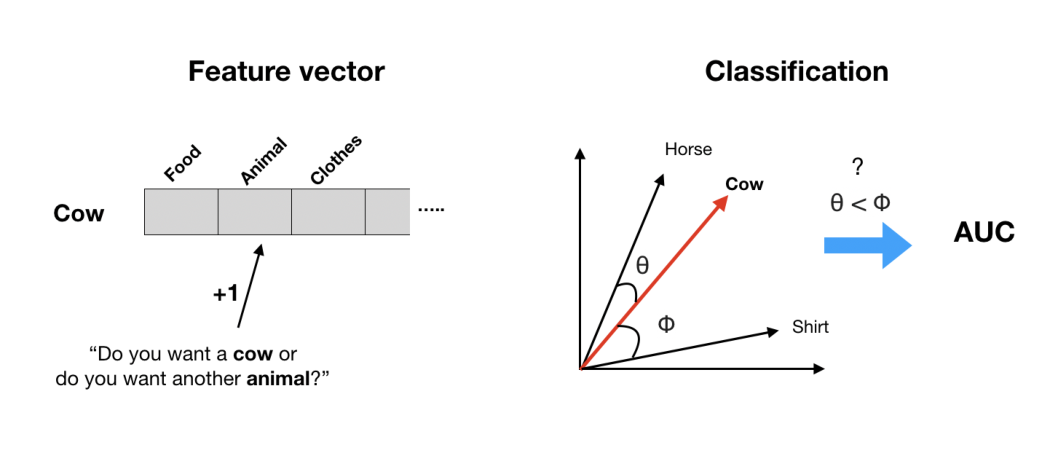
\includegraphics{child_language_journal_files/figure-latex/task-1} 

}

\caption{\label{fig:task} A schematic description of the task. For each basic-level word (here, `cow') a feature vector is derived from child-directed speech based on how the cue is defined. Here, the vector cells correspond to the superordinate categories. The entry in a given cell (e.g., animal) is incremented when the word `cow' co-occurs with the corresponding category label. The cue is evaluated based on its ability to classify pairs of words into 'same' or 'different' superordinate categories. Here, the pair `cow'-`horse' belongs to the same category. The corresponding vectors should be closer to each other than the vectors of a pair that belongs to different categories (e.g., `cow'-`shirt'). This evaluation is quantified by a standard measure in signal detection theory called the Area Under the ROC Curve (AUC).}\label{fig:task}
\end{figure}

\hypertarget{results}{%
\section{Results}\label{results}}

\hypertarget{individual-cue-results}{%
\subsection{Individual Cue Results}\label{individual-cue-results}}

Instances of the most explicit cue type, the \emph{\enquote{is-a-kind-of} cue}, were so rare that we could not even build feature vectors for basic-level words. In total, we found only four instances, all of them characterizing the \enquote{animal} category. Thus, we did not have meaningful results to report for this cue. As for the other cues, Figure \ref{fig:data-all} shows the global AUC score across categories as well as the AUC scores specific to each category.

\begin{figure}[h]

{\centering 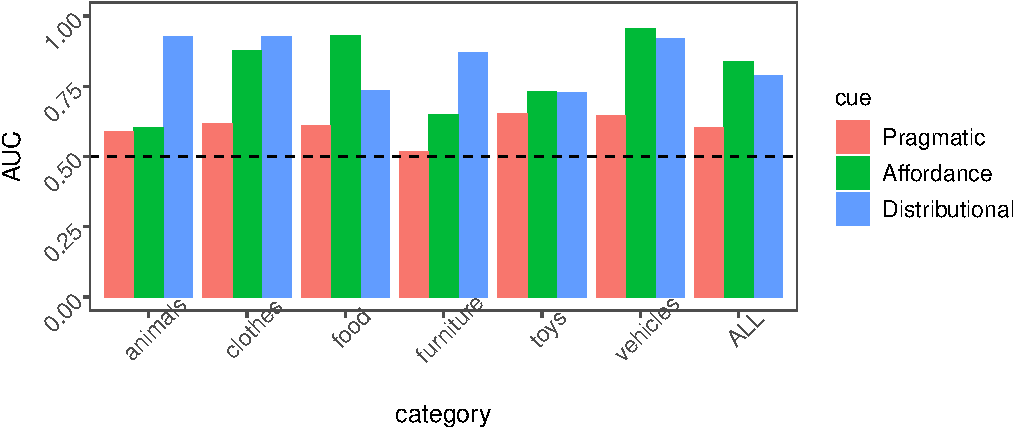
\includegraphics{child_language_journal_files/figure-latex/data-all-1} 

}

\caption{\label{fig:data-all} The Area Under the ROC Curve (AUC) scores of the cues for each category and across all categories ('ALL'). A value of 0.5 represents pure chance, and a value of 1 represents perfect performance.}\label{fig:data-all}
\end{figure}

The accuracy of the \emph{pragmatic cue} was generally low. For this cue, we only report the results with \(k=1\), which captures relations between basic and superordinate words within a single utterance. Increasing the value of \(k\) has led to worse, noisier performance. Regarding the \emph{affordance-based cue}, the accuracy was relatively high for some categories, i.e., \enquote{food}, \enquote{clothes}, \enquote{vehicles,} and \enquote{toys} and low for others, i.e., \enquote{furniture} and \enquote{animal.} Finally, the \emph{distributional cue} leads to the best overall results across most superordinate categories.

\hypertarget{developmental-change}{%
\subsection{Developmental change?}\label{developmental-change}}

The results above are based on child-directed speech up to three years old. As we mentioned earlier, this choice was based on research showing that this is the age when early signs of conceptual hierarchy emerge in children's lexicon. That said, several studies have documented changes in child-directed speech beyond 3 years (e.g., Jiang, Frank, Kulkarni, \& Fourtassi, 2022; Huttenlocher, Waterfall, Vasilyeva, Vevea, \& Hedges, 2010; Kunert, Fernández, \& Zuidema, 2011), and here we ask whether and how our linguistic cues undergo changes as children grow older and their linguistic input gets richer. While previous work does not make direct predictions about what could change regarding our specific cues, one can expect, e.g., that the distributional cue would become even stronger because the accumulation of more data in an increasing number of contexts would make more accurate the detection of shared patterns of co-occurrence. As for the pragmatic and affordance-based cues, we did not have a priori expectations about whether their role would become more or less important with development.

We followed the same approach as above but with data addressed to children up to 4, 5, and 6 years old, respectively. We stopped at 6 years old as this the age after which data become very sparse in the dataset CHILDES) (Table \ref{tab:development}). This cumulative way to study change (e.g., data up to 4 years old include data up to 3 years old) parallels the cumulative nature of children's linguistic experience. The results are summarized in Figure \ref{fig:dev}: They show that the performance of all cues remained stable across development (including for the distributional cue), suggesting that linguistic information in parental talk regarding conceptual hierarchy is already at ceiling by 3 years of age. More linguistic input does not change the informativeness of the cues.

\begin{table}[!htbp] \centering 
\caption{\label{tab:development} Information about the corpora used in the analysis of developmental change.}
\begin{tabularx}{\linewidth}{cXccXX}

\textbf{Age} & Age (months) & Children & Transcripts & Utterances & Words \\
\hline

\textbf{\textless4} & 30.1 & 843 & 6,750 & 2.657 M & 10.827 M\\

\textbf{\textless5} & 33.5 & 971 & 7,889 & 3.093 M & 12.807 M\\

\textbf{\textless6} & 34.8 & 1,046 & 8,654 & 3.221 M & 13.325 M\\

\hline
\end{tabularx}

\end{table}

\begin{figure}[!htbp]

{\centering 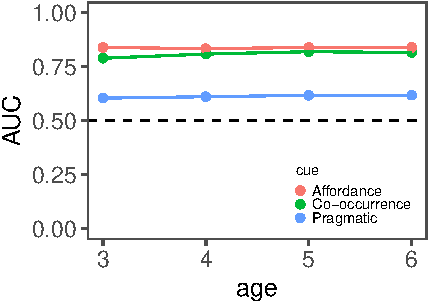
\includegraphics{child_language_journal_files/figure-latex/dev-1} 

}

\caption{\label{fig:dev} The Area Under the ROC Curve (AUC) scores for each cue (across all categories) using speech heard by children up to a particular age. A value of 0.5 represents pure chance, and a value of 1 represents perfect performance.}\label{fig:dev}
\end{figure}

\hypertarget{cross-cue-results}{%
\subsection{Cross-cue results}\label{cross-cue-results}}

The analyses above explored how the cues fare individually. Here we investigate the extent to which they provide complementary vs.~redundant information when combined. To this end, we fit six logistic regressions, one for each superordinate category. In all the regressions, the dependent variable was the binary classification of pairs of basic-level words belonging to same or different superordinate categories. The independent variables were the four similarity measures derived from the four cues. The results of the regressions,
summarized in Table \ref{tab:regressions}, indicate that, overall, each cue remains highly significant when controlling for the other cues. Thus, overall, the cues provided \emph{non-redundant} information to category membership.

\begin{table}[!htbp] \centering 
\caption{\label{tab:regressions} Logistic regressions predicting the binary classification of pairs of basic-level words as belonging to same or different superordinate categories. The predictors are the pairs' similarity measures derived from each cue. We fit a different regression for each superordinate category. The predictors were centered and scaled for comparability.} 
\label{} 
\begin{tabular}{@{\extracolsep{5pt}}lcccccc} 
\hline 
 & \multicolumn{4}{c}{} \\
 & (Intercept) & Distributional & Affordance & Pragmatic \\ 
\hline \\[-1.8ex] 
  Animals & $-$2.741$^{***}$ & 2.285$^{***}$ & 0.022 & 0.179$^{***}$\\
  & (0.085) & (0.074) & (0.057) & (0.050)\\
  & & & & & & \\
  Furniture & $-$3.195$^{***}$ & 2.040$^{***}$ & 0.547$^{***}$ & $-$0.104\\
  & (0.138) & (0.127) & (0.094) & (0.080) &\\
  & & & & & & \\
  Toys & $-$3.244$^{***}$ & 1.178$^{***}$ &  0.620$^{***}$ & 0.722$^{***}$\\
  & (0.155) & (0.136) & (0.113) & (0.120) &\\
  & & & & & & \\
  Food & $-$2.616$^{***}$ & 0.905$^{***}$ & 2.112$^{***}$ & 0.325$^{***}$\\
  & (0.112) & (0.060) & (0.092) & (0.059)\\
  & & & & & & \\
  Clothing & $-$3.101$^{***}$ & 1.644$^{***}$ & 1.535$^{***}$ & 0.359$^{*}$\\
  & (0.183) & (0.171) & (0.153) & (0.146)\\
  & & & & & & \\
  Vehicles & $-$4.663$^{***}$ & 1.249$^{***}$ & 2.211$^{***}$ & 0.159\\
  & (0.348) & (0.193) & (0.245) & (0.138)\\
  & & & & & & \\
 \\[-1.8ex] 

\hline \\[-1.8ex] 
\textit{Note:}  & \multicolumn{6}{r}{$^{*}$p$<$0.05; $^{**}$p$<$0.01; $^{***}$p$<$0.001} \\ 
\end{tabular} 
\end{table}

\hypertarget{discussion}{%
\section{Discussion}\label{discussion}}

A crucial question in the study of both language and cognitive development is understanding how children acquire the complex hierarchical relationships that characterize mature human semantic knowledge. A particularly challenging task is learning how basic-level terms are related to abstract superordinate concepts. One difficulty of this task stems from the fact that first-hand perceptual experience does not always provide direct evidence for learning, e.g., superordinate category, in particular, often requires additional social input that indicates how the child's specific linguistic community carves up the world into concepts (e.g., Waddy, 1982, Gelman (2009); Harris, 2012, Csibra and Gergely (2009)). The current work is a first step to investigating the extent to which \emph{language} that children hear around them can provide explicit or implicit cues about conceptual hierarchy. The main novelty of our work is that we used a unified computational framework that has allowed us to directly compare the relative importance of different linguistic cues present in child-directed speech with respect to their ability to help learn the taxonomic relations linking basic-level words in children's emerging lexicon to six common superordinate categories.

\hypertarget{the-relative-usefulness-of-cues-to-conceptual-hierarchy-in-child-directed-speech}{%
\subsection{The relative usefulness of cues to conceptual hierarchy in child-directed speech}\label{the-relative-usefulness-of-cues-to-conceptual-hierarchy-in-child-directed-speech}}

The most explicit cue -- where caregivers state the relationship between a basic-level term and its superordinate category label (e.g., \enquote{a dog is a kind of animal}) -- did not scale up well to the naturalistic dataset we used. This finding contrasts with previous work that found this cue in parental speech (Callanan, 1985; Shipley et al., 1983). This contrast can be explained by the fact that these previous studies were done in the context of rather controlled settings and parents were aware of the task (e.g., teaching words at the superordinate level), whereas here we tested a corpus of largely \emph{spontaneous} speech.

Caregivers can hint at conceptual hierarchy without necessarily stating it explicitly, however (see Table 1). To capture this pragmatic cue, we quantified the co-occurrence between basic-level and superordinate terms within utterances. This simple operationalization was meant to capture all possible ways the hierarchical relationship between two concepts can be expressed linguistically. However, it also made the representation susceptible to errors, mainly by increasing the rate of false alarms: A basic level term (e.g., \enquote{juice}) can also co-occur with a superordinate label of which it is not an instance (e.g., \enquote{Don't pour the juice on your clothes!}). The rate of such false alarms was quite high, which explains the overall low -- though not random -- scores of this cue.

From a developmental point of view, this finding highlights the limitation (at scale) of a simple co-occurrence-based strategy: A deeper understanding of the meaning of the utterance is necessary if children are to learn conceptual hierarchy from pragmatic cues while avoiding false alarms. Future work should aim at providing a more refined computational implementation of these cues. While the ability of state-of-the-art language models in making general, reliable pragmatic inference is still poor, modeling work in Natural Language Processing that has focused on the specific task of inferring taxonomic relations from textual data has been more fruitful (e.g., Chami, Abu-El-Haija, Perozzi, Ré, \& Murphy, 2022; Le, Roller, Papaxanthos, Kiela, \& Nickel, 2019; Zhang et al., 2022). While this literature has not yet managed to reliably extract taxonomic relations from pairs of terms in a sentence when the relation is not linguistically explicit (i.e., as defined in the pragmatic cue), the methods developed -- when relevant and cognitively plausible -- can be a source of inspiration for researchers in child development to improve the study of children's linguistic input in terms of inferring conceptual structure more generally.

Another linguistic cue we tested is based on affordances (e.g., basic-level terms for food are \enquote{eat}-able and can be detected as such if they occur as the grammatical object of the verb \enquote{eat}). The accuracy of the affordance-based cue was relatively high for the categories which had an obvious verb to cue its affordance, i.e., \enquote{food} (eat), \enquote{clothes} (wear), \enquote{vehicles} (ride), and \enquote{toys} (play). The accuracy was low in the case of \enquote{furniture} since the verb \enquote{use} is not exclusive to this category and can also be used with instances of other categories, leading to false alarms. The accuracy for \enquote{animal} was also low as it was not characterized by any particular verb. \footnote{At the same time, the performance of the cue on this category was not totally random because animal instances tend to co-occur more consistently with some verbs from other categories (e.g., "ride a horse", "play with the dog", and "eat the chicken").}

Finally, the pure distributional cue was the most implicit one since it did not rely on a label or any other linguistic marker for the abstract category. The score for this cue was generally high, including for \enquote{animal} and \enquote{furniture,} two categories that were not reliably captured with any of the previous cues. This finding suggests that children can learn that certain basic-level terms share common abstract properties by realizing that they have a similar distribution in speech, i.e., that they are used in similar linguistic contexts. This strategy could be even more useful for high-level categories that do not have an explicit label, or for which the label could not be available to the young learners (e.g., \enquote{animate} vs. \enquote{inanimate}).

In addition to these insights obtained by testing each cue individually, we also tested how the cues interact with one another when they were all combined to predict learning in each superordinate category. We found that the cues were largely non-redundant across most categories, suggesting that children can combine several cues to complement their learning. Further, the cues did not fare similarly across categories, suggesting that children can rely more on different cues to learn different categories, e.g., they may use the affordance-based cue more to learn about \enquote{food}, \enquote{clothes} or \enquote{vehicle} and the distributional cue more to learn about \enquote{animals} and \enquote{furniture.} For example, early on, children can learn that some words tend to occur as objects to the verbs \enquote{eat,} \enquote{wear,} or \enquote{ride.} enhancing the learning of these conceptual links. In parallel, and as they accumulate more linguistic experience, they develop increasingly more accurate statistical patterns about which pairs of words share similar distribution in speech, leading to increasingly more refined knowledge about the categories \enquote{animals} and \enquote{furniture.}

\hypertarget{possible-learning-mechanisms}{%
\subsection{Possible learning mechanisms}\label{possible-learning-mechanisms}}

For all the cues discussed above, our goal was to test their ability to provide a reliable source of information in child-directed speech. However, our instantiation of the cues abstracted away from the children's cognitive and information processing limitations, providing only an \enquote{ideal observer} point of view (Marr, 1982). That said, several experimental studies have provided evidence for the cognitive plausibility of the learning mechanisms that underlie each of these cues.

For instance, preschool children ably use the \enquote{is-a-kind-of} cue to interpret the meaning of a novel word at the superordinate level (Callanan, 1989) (though the current study shows this cue to be highly impoverished in natural input). Both the pragmatic and affordance-based cues rely on the ability to track co-occurrence between pairs of words: the basic- vs.~superordinate-level labels in the former and the basic-level label vs.~the verb cueing affordance in the latter. Extensive research in the last couple of decades has shown that even infants are capable of tracking the co-occurrence of various linguistic units (Saffran, Aslin, \& Newport, 1996). In particular, Bannard \& Matthews (2008) have shown toddlers encode together in memory collocational words such as \enquote{sit} and \enquote{chair} and Wojcik \& Saffran (2015) have shown that they encode relationships between novel words co-occurring in a sentence. The distributional cue, on the other hand, requires not only sensitivity to word co-occurrence (as with the pragmatic and affordance-based cues) but also sensitivity to the words' \emph{shared} patterns of co-occurrence. For example, learners should be sensitive to the fact that \enquote{raven} and \enquote{salmon} co-occur with similar words and phrases such as \enquote{lay egg}, \enquote{live,} and \enquote{reproduce}, although the pair of words \enquote{raven} and \enquote{salmon} may not themselves co-occur with each other. There is some evidence that even infants are sensitive to shared patterns of co-occurrence (e.g., Lany \& Saffran, 2011).

Note, however, that while the detection of reliably co-occurring pair of labels can create a mental association (via simple associative mechanisms), it is not clear how this association would develop into becoming a taxonomic relation (as opposed to, say, a thematic relation). In other words, detecting co-occurrence is a necessary but not a sufficient condition for the learning of conceptual \emph{hierarchy}. To make full advantage of the affordance-based cue, it is important to also understand the syntactic relations (i.e., verb-complement structure). For the pragmatic cue, it is crucial to also make inferences about the speaker's intended relationship between basic and superordinate terms given the context. Indeed, the fact that our simple implementation of the pragmatic cue based on mere co-occurrence has led to poor performance is a strong testimony to the need for this additional, higher-level inference.

As for the pure distributional cue, and when operating alone, there is a priori no additional information (syntactic or extra-linguistic) that can help children induce conceptual hierarchy beyond information about word co-occurrence. On this account, the accumulation of direct co-occurrence in children's memory (e.g., \enquote{fruits}-\enquote{hungry} and \enquote{vegetables}-\enquote{hungry}) leads to the realization (perhaps triggered by cognitive maturation, e.g., Bauer \& San Souci (2010); Savic, Unger, \& Sloutsky (2022)) that some words share similar pattern of co-occurrence (e.g., that \enquote{fruits} and \enquote{vegetables} co-occur in similar linguistic contexts; in this example, they both co-occur with \enquote{hungry}), which then foster the creation of a taxonomic -- rather than a thematic -- link (i.e., \enquote{fruits} and \enquote{vegetables} are instances of a single higher-level conceptual category, e.g., \enquote{food}) (Brown \& Berko, 1960; Ervin, 1961; McNeill, 1963; Sloutsky et al., 2017). It is still not entirely unclear what precise mechanistic process can explain how sensitivity to shared patterns of co-occurrence between two labels may give rise to a taxonomic link relating these labels to a single superordinate category, supporting conceptual inference and knowledge generalization, but we refer the reader to Unger \& Fisher (2021) and Savic et al. (2022) for a review and discussion of some hypothesized mechanisms based on behavioral, computational, and/or neuroscientific evidence.

\hypertarget{conclusion-and-future-work}{%
\subsection{Conclusion and future work}\label{conclusion-and-future-work}}

This work studied how toddlers begin to acquire conceptual hierarchy. While most previous work focused on the role of first-hand observation, here we investigated another (complementary) source of input, i.e., the language children hear around them. We found implicit cues (the affordance-based and distributional cues) to be much more reliable than explicit cues (\enquote{is-a-kind-of} and pragmatic cues). While studies have shown that children are cognitively equipped to learn conceptual hierarchy equally from both implicit and explicit cues, our input analysis suggests that implicit cues could be the more important source of this knowledge.

That said, the current work is only a first step and more work is needed to refine the cues, especially the ones for which we only provided a simple approximation such as the pragmatic cue. In addition, while we emphasized the complementary aspect of linguistic cues compared to perceptual cues, future work should allow direct comparison between these two accounts in order to better estimate the relative role of each source of information in development (e.g., Andrews, Frank, \& Vigliocco, 2014; Bruni, Tran, \& Baroni, 2014). Ultimately, the goal would be to integrate both sources into a \emph{cognitive} model that uses these cues in a principle way. Such a model should make precise developmental predictions about how the cues interact and how their role in learning changes across development.

Another direction for future work is to compare the findings we obtained with data in English to other languages. Understanding variation in children's experiences allows us to determine which aspects of development are universal and which are culture-specific (Rogoff, Dahl, \& Callanan, 2018). The learning of conceptual hierarchy is an excellent case stud; we know for example that superordinate concepts have both similarities and differences across cultures (e.g. Waddy, 1982). In addition, the cues may vary in terms of their reliability from one language to the other, depending both on cultural practices/parenting styles and on the specificities of the language. Finally, it is crucial for future work to investigate whether and how variation in caregivers' language induces variations in children's conceptualization of the world.

\hypertarget{references}{%
\section{References}\label{references}}

\setlength{\parindent}{-0.5in}
\setlength{\leftskip}{0.5in}

\hypertarget{refs}{}
\leavevmode\hypertarget{ref-andrews2014}{}%
Andrews, M., Frank, S., \& Vigliocco, G. (2014). Reconciling embodied and distributional accounts of meaning in language. \emph{Topics in Cognitive Science}, \emph{6}(3), 359--370.

\leavevmode\hypertarget{ref-andrews2009integrating}{}%
Andrews, M., Vigliocco, G., \& Vinson, D. (2009). Integrating experiential and distributional data to learn semantic representations. \emph{Psychological Review}, \emph{116}(3), 463.

\leavevmode\hypertarget{ref-bannard2008}{}%
Bannard, C., \& Matthews, D. (2008). Stored word sequences in language learning: The effect of familiarity on children's repetition of four-word combinations. \emph{Psychological Science}, \emph{19}(3), 241--248.

\leavevmode\hypertarget{ref-bauer2010going}{}%
Bauer, P. J., \& San Souci, P. (2010). Going beyond the facts: Young children extend knowledge by integrating episodes. \emph{Journal of Experimental Child Psychology}, \emph{107}(4), 452--465.

\leavevmode\hypertarget{ref-blaye2006categorical}{}%
Blaye, A., Bernard-Peyron, V., Paour, J.-L., \& Bonthoux, F. (2006). Categorical flexibility in children: Distinguishing response flexibility from conceptual flexibility; the protracted development of taxonomic representations. \emph{European Journal of Developmental Psychology}, \emph{3}(2), 163--188.

\leavevmode\hypertarget{ref-brown1960word}{}%
Brown, R., \& Berko, J. (1960). Word association and the acquisition of grammar. \emph{Child Development}, 1--14.

\leavevmode\hypertarget{ref-bruni2014}{}%
Bruni, E., Tran, N.-K., \& Baroni, M. (2014). Multimodal distributional semantics. \emph{Journal of Artificial Intelligence Research}, \emph{49}, 1--47.

\leavevmode\hypertarget{ref-callanan1985}{}%
Callanan, M. A. (1985). How parents label objects for young children: The role of input in the acquisition of category hierarchies. \emph{Child Development}, 508--523.

\leavevmode\hypertarget{ref-callanan1989}{}%
Callanan, M. A. (1989). Development of object categories and inclusion relations: Preschoolers' hypotheses about word meanings. \emph{Developmental Psychology}, \emph{25}(2).

\leavevmode\hypertarget{ref-carey1987}{}%
Carey, S. (1987). \emph{Conceptual change in childhood}. MIT Press.

\leavevmode\hypertarget{ref-chami2022machine}{}%
Chami, I., Abu-El-Haija, S., Perozzi, B., Ré, C., \& Murphy, K. (2022). Machine learning on graphs: A model and comprehensive taxonomy. \emph{Journal of Machine Learning Research}, \emph{23}(89), 1--64.

\leavevmode\hypertarget{ref-chi1989}{}%
Chi, M. T., Hutchinson, J. E., \& Robin, A. F. (1989). How inferences about novel domain-related concepts can be constrained by structured knowledge. \emph{Merrill-Palmer Quarterly (1982-)}, 27--62.

\leavevmode\hypertarget{ref-clark1997}{}%
Clark, E. V. (1997). Conceptual perspective and lexical choice in acquisition. \emph{Cognition}, \emph{64}(1), 1--37.

\leavevmode\hypertarget{ref-csibra2009}{}%
Csibra, G., \& Gergely, G. (2009). Natural pedagogy. \emph{Trends in Cognitive Sciences}, \emph{13}(4), 148--153.

\leavevmode\hypertarget{ref-ervin1961changes}{}%
Ervin, S. M. (1961). Changes with age in the verbal determinants of word-association. \emph{The American Journal of Psychology}, \emph{74}(3), 361--372.

\leavevmode\hypertarget{ref-fenson94}{}%
Fenson, L., Dale, P. S., Reznick, J. S., Bates, E., Thal, D. J., Pethick, S. J., \ldots{} Stiles, J. (1994). Variability in early communicative development. \emph{Monographs of the Society for Research in Child Development}, \emph{59}(5), i--185.

\leavevmode\hypertarget{ref-fourtassi2020word}{}%
Fourtassi, A. (2020). Word co-occurrence in child-directed speech predicts children's free word associations. In \emph{Proceedings of the workshop on cognitive modeling and computational linguistics} (pp. 49--53).

\leavevmode\hypertarget{ref-fourtassi2014}{}%
Fourtassi, A., Dunbar, E., \& Dupoux, E. (2014). Self-consistency as an inductive bias in early language acquisition. In \emph{Proceedings of the annual meeting of the cognitive science society} (Vol. 36).

\leavevmode\hypertarget{ref-fourtassi2013}{}%
Fourtassi, A., \& Dupoux, E. (2013). A corpus-based evaluation method for distributional semantic models. In \emph{51st annual meeting of the association for computational linguistics proceedings of the student research workshop} (pp. 165--171).

\leavevmode\hypertarget{ref-fourtassi2019}{}%
Fourtassi, A., Scheinfeld, I., \& Frank, M. C. (2019). The development of abstract concepts in children's early lexical networks. In \emph{Proceedings of the workshop on cognitive modeling and computational linguistics} (pp. 129--133).

\leavevmode\hypertarget{ref-frank2021variability}{}%
Frank, M. C., Braginsky, M., Yurovsky, D., \& Marchman, V. A. (2021). \emph{Variability and consistency in early language learning: The wordbank project}. MIT Press.

\leavevmode\hypertarget{ref-frermann2016}{}%
Frermann, L., \& Lapata, M. (2016a). Incremental bayesian category learning from natural language. \emph{Cognitive Science}, \emph{40}(6), 1333--1381.

\leavevmode\hypertarget{ref-frermann2016incremental}{}%
Frermann, L., \& Lapata, M. (2016b). Incremental bayesian category learning from natural language. \emph{Cognitive Science}, \emph{40}(6), 1333--1381.

\leavevmode\hypertarget{ref-gelman2009}{}%
Gelman, S. A. (2009). Learning from others: Children's construction of concepts. \emph{Annual Review of Psychology}, \emph{60}, 115--140.

\leavevmode\hypertarget{ref-gentner1999comparison}{}%
Gentner, D., \& Namy, L. L. (1999). Comparison in the development of categories. \emph{Cognitive Development}, \emph{14}(4), 487--513.

\leavevmode\hypertarget{ref-harris2012}{}%
Harris, P. L. (2012). \emph{Trusting what you're told}. Harvard University Press.

\leavevmode\hypertarget{ref-harris1957}{}%
Harris, Z. S. (1957). Co-occurrence and transformation in linguistic structure. \emph{Language}, \emph{33}(3).

\leavevmode\hypertarget{ref-hills2010}{}%
Hills, T. T., Maouene, J., Riordan, B., \& Smith, L. B. (2010). The associative structure of language: Contextual diversity in early word learning. \emph{Journal of Memory and Language}, \emph{63}(3), 259--273.

\leavevmode\hypertarget{ref-huebner2018}{}%
Huebner, P. A., \& Willits, J. A. (2018). Structured semantic knowledge can emerge automatically from predicting word sequences in child-directed speech. \emph{Frontiers in Psychology}, \emph{9}, 133.

\leavevmode\hypertarget{ref-huttenlocher2010sources}{}%
Huttenlocher, J., Waterfall, H., Vasilyeva, M., Vevea, J., \& Hedges, L. V. (2010). Sources of variability in children's language growth. \emph{Cognitive Psychology}, \emph{61}(4), 343--365.

\leavevmode\hypertarget{ref-inagaki2002}{}%
Inagaki, K., \& Hatano, Giyoo. (2002). \emph{Young children's naive thinking about the biological world}. New York : Psychology Press.

\leavevmode\hypertarget{ref-inhelder2013}{}%
Inhelder, B., \& Piaget, J. (2013). \emph{The early growth of logic in the child: Classification and seriation}. Routledge.

\leavevmode\hypertarget{ref-jiang2022exploring}{}%
Jiang, H., Frank, M. C., Kulkarni, V., \& Fourtassi, A. (2022). Exploring patterns of stability and change in caregivers' word usage across early childhood. \emph{Cognitive Science}, \emph{46}(7), e13177.

\leavevmode\hypertarget{ref-kemp2007learning}{}%
Kemp, C., Perfors, A., \& Tenenbaum, J. B. (2007). Learning overhypotheses with hierarchical bayesian models. \emph{Developmental Science}, \emph{10}(3), 307--321.

\leavevmode\hypertarget{ref-kunert2011adaptation}{}%
Kunert, R., Fernández, R., \& Zuidema, W. (2011). Adaptation in child directed speech: Evidence from corpora. \emph{Proc. SemDial}, 112--119.

\leavevmode\hypertarget{ref-landauer1997solution}{}%
Landauer, T. K., \& Dumais, S. T. (1997). A solution to plato's problem: The latent semantic analysis theory of acquisition, induction, and representation of knowledge. \emph{Psychological Review}, \emph{104}(2), 211.

\leavevmode\hypertarget{ref-lany2011}{}%
Lany, J., \& Saffran, J. R. (2011). Interactions between statistical and semantic information in infant language development. \emph{Developmental Science}, \emph{14}(5), 1207--1219.

\leavevmode\hypertarget{ref-le2019inferring}{}%
Le, M., Roller, S., Papaxanthos, L., Kiela, D., \& Nickel, M. (2019). Inferring concept hierarchies from text corpora via hyperbolic embeddings. In \emph{Proceedings of the 57th annual meeting of the association for computational linguistics} (pp. 3231--3241).

\leavevmode\hypertarget{ref-liu2001}{}%
Liu, J., Golinkoff, R. M., \& Sak, K. (2001). One cow does not an animal make: Young children can extend novel words at the superordinate level. \emph{Child Development}, \emph{72}(6), 1674--1694.

\leavevmode\hypertarget{ref-lucariello1992taxonomic}{}%
Lucariello, J., Kyratzis, A., \& Nelson, K. (1992). Taxonomic knowledge: What kind and when? \emph{Child Development}, \emph{63}(4), 978--998.

\leavevmode\hypertarget{ref-macwhinney2000}{}%
MacWhinney, B. (2000). \emph{The childes project: Tools for analyzing talk. Transcription format and programs} (Vol. 1). Psychology Press.

\leavevmode\hypertarget{ref-madole1999}{}%
Madole, K. L., \& Oakes, L. M. (1999). Making sense of infant categorization: Stable processes and changing representations. \emph{Developmental Review}, \emph{19}(2), 263--296.

\leavevmode\hypertarget{ref-markman1989}{}%
Markman, E. M. (1989). \emph{Categorization and naming in children: Problems of induction}. MIT Press.

\leavevmode\hypertarget{ref-markman1984children}{}%
Markman, E. M., \& Hutchinson, J. E. (1984). Children's sensitivity to constraints on word meaning: Taxonomic versus thematic relations. \emph{Cognitive Psychology}, \emph{16}(1), 1--27.

\leavevmode\hypertarget{ref-marr1982}{}%
Marr, D. (1982). \emph{Vision: A computational investigation into the human representation and processing of visual information}. Henry Holt; Co., Inc.

\leavevmode\hypertarget{ref-mcclelland2003}{}%
McClelland, J. L., \& Rogers, T. T. (2003). The parallel distributed processing approach to semantic cognition. \emph{Nature Reviews Neuroscience}, \emph{4}(4), 310--322.

\leavevmode\hypertarget{ref-mcneill1963origin}{}%
McNeill, D. (1963). The origin of associations within the same grammatical class. \emph{Journal of Verbal Learning and Verbal Behavior}, \emph{2}(3), 250--262.

\leavevmode\hypertarget{ref-mikolov2013}{}%
Mikolov, T., Sutskever, I., Chen, K., Corrado, G. S., \& Dean, J. (2013). Distributed representations of words and phrases and their compositionality. In \emph{Advances in neural information processing systems} (pp. 3111--3119).

\leavevmode\hypertarget{ref-murphy2004big}{}%
Murphy, G. (2004). \emph{The big book of concepts}. MIT press.

\leavevmode\hypertarget{ref-quinn2000}{}%
Quinn, P. C., \& Eimas, P. D. (2000). The emergence of category representations during infancy: Are separate perceptual and conceptual processes required? \emph{Journal of Cognition and Development}, \emph{1}(1), 55--61.

\leavevmode\hypertarget{ref-rogoff2018}{}%
Rogoff, B., Dahl, A., \& Callanan, M. (2018). The importance of understanding children's lived experience. \emph{Developmental Review}, \emph{50}, 5--15.

\leavevmode\hypertarget{ref-saffran1996}{}%
Saffran, J. R., Aslin, R. N., \& Newport, E. L. (1996). Statistical learning by 8-month-old infants. \emph{Science}, \emph{274}(5294), 1926--1928.

\leavevmode\hypertarget{ref-sanchez2019}{}%
Sanchez, A., Meylan, S. C., Braginsky, M., MacDonald, K. E., Yurovsky, D., \& Frank, M. C. (2019). Childes-db: A flexible and reproducible interface to the child language data exchange system. \emph{Behavior Research Methods}, \emph{51}(4), 1928--1941.

\leavevmode\hypertarget{ref-savic2022experience}{}%
Savic, O., Unger, L., \& Sloutsky, V. M. (2022). Experience and maturation: The contribution of co-occurrence regularities in language to the development of semantic organization. \emph{Child Development}.

\leavevmode\hypertarget{ref-saxe2019mathematical}{}%
Saxe, A. M., McClelland, J. L., \& Ganguli, S. (2019). A mathematical theory of semantic development in deep neural networks. \emph{Proceedings of the National Academy of Sciences}, \emph{116}(23), 11537--11546.

\leavevmode\hypertarget{ref-shipley1983}{}%
Shipley, E. F., Kuhn, I. F., \& Madden, E. C. (1983). Mothers' use of superordinate category terms. \emph{Journal of Child Language}, \emph{10}(3).

\leavevmode\hypertarget{ref-sloutsky2015}{}%
Sloutsky, V. (2015). Conceptual development. \emph{Handbook of Child Psychology and Developmental Science}, 1--50.

\leavevmode\hypertarget{ref-sloutsky2010}{}%
Sloutsky, V. M. (2010). From perceptual categories to concepts: What develops? \emph{Cognitive Science}, \emph{34}(7), 1244--1286.

\leavevmode\hypertarget{ref-sloutsky2017}{}%
Sloutsky, V. M., Yim, H., Yao, X., \& Dennis, S. (2017). An associative account of the development of word learning. \emph{Cognitive Psychology}, \emph{97}, 1--30.

\leavevmode\hypertarget{ref-smith1992}{}%
Smith, L. B., \& Heise, D. (1992). Perceptual similarity and conceptual structure. In \emph{Advances in psychology} (Vol. 93, pp. 233--272).

\leavevmode\hypertarget{ref-stella2017}{}%
Stella, M., Beckage, N. M., \& Brede, M. (2017). Multiplex lexical networks reveal patterns in early word acquisition in children. \emph{Scientific Reports}, \emph{7}.

\leavevmode\hypertarget{ref-tenenbaum2006theory}{}%
Tenenbaum, J. B., Griffiths, T. L., \& Kemp, C. (2006). Theory-based bayesian models of inductive learning and reasoning. \emph{Trends in Cognitive Sciences}, \emph{10}(7), 309--318.

\leavevmode\hypertarget{ref-unger2021}{}%
Unger, L., \& Fisher, A. V. (2021). The emergence of richly organized semantic knowledge from simple statistics: A synthetic review. \emph{Developmental Review}, \emph{60}, 100949.

\leavevmode\hypertarget{ref-unger2020statistical}{}%
Unger, L., Savic, O., \& Sloutsky, V. M. (2020). Statistical regularities shape semantic organization throughout development. \emph{Cognition}, \emph{198}, 104190.

\leavevmode\hypertarget{ref-waddy1982}{}%
Waddy, J. A. (1982). Biological classification from a groote eylandt aborigine's point of view. \emph{Journal of Ethnobiology}, \emph{2}(1), 63--77.

\leavevmode\hypertarget{ref-winer1980class}{}%
Winer, G. A. (1980). Class-inclusion reasoning in children: A review of the empirical literature. \emph{Child Development}, 309--328.

\leavevmode\hypertarget{ref-wojcik2015}{}%
Wojcik, E. H., \& Saffran, J. R. (2015). Toddlers encode similarities among novel words from meaningful sentences. \emph{Cognition}, \emph{138}, 10--20.

\leavevmode\hypertarget{ref-xu2007word}{}%
Xu, F., \& Tenenbaum, J. B. (2007). Word learning as bayesian inference. \emph{Psychological Review}, \emph{114}(2), 245.

\leavevmode\hypertarget{ref-zhang2022aser}{}%
Zhang, H., Liu, X., Pan, H., Ke, H., Ou, J., Fang, T., \& Song, Y. (2022). Aser: Towards large-scale commonsense knowledge acquisition via higher-order selectional preference over eventualities. \emph{Artificial Intelligence}, 103740.

\leavevmode\hypertarget{ref-andrews2014}{}%
Andrews, M., Frank, S., \& Vigliocco, G. (2014). Reconciling embodied and distributional accounts of meaning in language. \emph{Topics in Cognitive Science}, \emph{6}(3), 359--370.

\leavevmode\hypertarget{ref-andrews2009integrating}{}%
Andrews, M., Vigliocco, G., \& Vinson, D. (2009). Integrating experiential and distributional data to learn semantic representations. \emph{Psychological Review}, \emph{116}(3), 463.

\leavevmode\hypertarget{ref-bannard2008}{}%
Bannard, C., \& Matthews, D. (2008). Stored word sequences in language learning: The effect of familiarity on children's repetition of four-word combinations. \emph{Psychological Science}, \emph{19}(3), 241--248.

\leavevmode\hypertarget{ref-bauer2010going}{}%
Bauer, P. J., \& San Souci, P. (2010). Going beyond the facts: Young children extend knowledge by integrating episodes. \emph{Journal of Experimental Child Psychology}, \emph{107}(4), 452--465.

\leavevmode\hypertarget{ref-blaye2006categorical}{}%
Blaye, A., Bernard-Peyron, V., Paour, J.-L., \& Bonthoux, F. (2006). Categorical flexibility in children: Distinguishing response flexibility from conceptual flexibility; the protracted development of taxonomic representations. \emph{European Journal of Developmental Psychology}, \emph{3}(2), 163--188.

\leavevmode\hypertarget{ref-brown1960word}{}%
Brown, R., \& Berko, J. (1960). Word association and the acquisition of grammar. \emph{Child Development}, 1--14.

\leavevmode\hypertarget{ref-bruni2014}{}%
Bruni, E., Tran, N.-K., \& Baroni, M. (2014). Multimodal distributional semantics. \emph{Journal of Artificial Intelligence Research}, \emph{49}, 1--47.

\leavevmode\hypertarget{ref-callanan1985}{}%
Callanan, M. A. (1985). How parents label objects for young children: The role of input in the acquisition of category hierarchies. \emph{Child Development}, 508--523.

\leavevmode\hypertarget{ref-callanan1989}{}%
Callanan, M. A. (1989). Development of object categories and inclusion relations: Preschoolers' hypotheses about word meanings. \emph{Developmental Psychology}, \emph{25}(2).

\leavevmode\hypertarget{ref-carey1987}{}%
Carey, S. (1987). \emph{Conceptual change in childhood}. MIT Press.

\leavevmode\hypertarget{ref-chami2022machine}{}%
Chami, I., Abu-El-Haija, S., Perozzi, B., Ré, C., \& Murphy, K. (2022). Machine learning on graphs: A model and comprehensive taxonomy. \emph{Journal of Machine Learning Research}, \emph{23}(89), 1--64.

\leavevmode\hypertarget{ref-chi1989}{}%
Chi, M. T., Hutchinson, J. E., \& Robin, A. F. (1989). How inferences about novel domain-related concepts can be constrained by structured knowledge. \emph{Merrill-Palmer Quarterly (1982-)}, 27--62.

\leavevmode\hypertarget{ref-clark1997}{}%
Clark, E. V. (1997). Conceptual perspective and lexical choice in acquisition. \emph{Cognition}, \emph{64}(1), 1--37.

\leavevmode\hypertarget{ref-csibra2009}{}%
Csibra, G., \& Gergely, G. (2009). Natural pedagogy. \emph{Trends in Cognitive Sciences}, \emph{13}(4), 148--153.

\leavevmode\hypertarget{ref-ervin1961changes}{}%
Ervin, S. M. (1961). Changes with age in the verbal determinants of word-association. \emph{The American Journal of Psychology}, \emph{74}(3), 361--372.

\leavevmode\hypertarget{ref-fenson94}{}%
Fenson, L., Dale, P. S., Reznick, J. S., Bates, E., Thal, D. J., Pethick, S. J., \ldots{} Stiles, J. (1994). Variability in early communicative development. \emph{Monographs of the Society for Research in Child Development}, \emph{59}(5), i--185.

\leavevmode\hypertarget{ref-fourtassi2020word}{}%
Fourtassi, A. (2020). Word co-occurrence in child-directed speech predicts children's free word associations. In \emph{Proceedings of the workshop on cognitive modeling and computational linguistics} (pp. 49--53).

\leavevmode\hypertarget{ref-fourtassi2014}{}%
Fourtassi, A., Dunbar, E., \& Dupoux, E. (2014). Self-consistency as an inductive bias in early language acquisition. In \emph{Proceedings of the annual meeting of the cognitive science society} (Vol. 36).

\leavevmode\hypertarget{ref-fourtassi2013}{}%
Fourtassi, A., \& Dupoux, E. (2013). A corpus-based evaluation method for distributional semantic models. In \emph{51st annual meeting of the association for computational linguistics proceedings of the student research workshop} (pp. 165--171).

\leavevmode\hypertarget{ref-fourtassi2019}{}%
Fourtassi, A., Scheinfeld, I., \& Frank, M. C. (2019). The development of abstract concepts in children's early lexical networks. In \emph{Proceedings of the workshop on cognitive modeling and computational linguistics} (pp. 129--133).

\leavevmode\hypertarget{ref-frank2021variability}{}%
Frank, M. C., Braginsky, M., Yurovsky, D., \& Marchman, V. A. (2021). \emph{Variability and consistency in early language learning: The wordbank project}. MIT Press.

\leavevmode\hypertarget{ref-frermann2016}{}%
Frermann, L., \& Lapata, M. (2016a). Incremental bayesian category learning from natural language. \emph{Cognitive Science}, \emph{40}(6), 1333--1381.

\leavevmode\hypertarget{ref-frermann2016incremental}{}%
Frermann, L., \& Lapata, M. (2016b). Incremental bayesian category learning from natural language. \emph{Cognitive Science}, \emph{40}(6), 1333--1381.

\leavevmode\hypertarget{ref-gelman2009}{}%
Gelman, S. A. (2009). Learning from others: Children's construction of concepts. \emph{Annual Review of Psychology}, \emph{60}, 115--140.

\leavevmode\hypertarget{ref-gentner1999comparison}{}%
Gentner, D., \& Namy, L. L. (1999). Comparison in the development of categories. \emph{Cognitive Development}, \emph{14}(4), 487--513.

\leavevmode\hypertarget{ref-harris2012}{}%
Harris, P. L. (2012). \emph{Trusting what you're told}. Harvard University Press.

\leavevmode\hypertarget{ref-harris1957}{}%
Harris, Z. S. (1957). Co-occurrence and transformation in linguistic structure. \emph{Language}, \emph{33}(3).

\leavevmode\hypertarget{ref-hills2010}{}%
Hills, T. T., Maouene, J., Riordan, B., \& Smith, L. B. (2010). The associative structure of language: Contextual diversity in early word learning. \emph{Journal of Memory and Language}, \emph{63}(3), 259--273.

\leavevmode\hypertarget{ref-huebner2018}{}%
Huebner, P. A., \& Willits, J. A. (2018). Structured semantic knowledge can emerge automatically from predicting word sequences in child-directed speech. \emph{Frontiers in Psychology}, \emph{9}, 133.

\leavevmode\hypertarget{ref-huttenlocher2010sources}{}%
Huttenlocher, J., Waterfall, H., Vasilyeva, M., Vevea, J., \& Hedges, L. V. (2010). Sources of variability in children's language growth. \emph{Cognitive Psychology}, \emph{61}(4), 343--365.

\leavevmode\hypertarget{ref-inagaki2002}{}%
Inagaki, K., \& Hatano, Giyoo. (2002). \emph{Young children's naive thinking about the biological world}. New York : Psychology Press.

\leavevmode\hypertarget{ref-inhelder2013}{}%
Inhelder, B., \& Piaget, J. (2013). \emph{The early growth of logic in the child: Classification and seriation}. Routledge.

\leavevmode\hypertarget{ref-jiang2022exploring}{}%
Jiang, H., Frank, M. C., Kulkarni, V., \& Fourtassi, A. (2022). Exploring patterns of stability and change in caregivers' word usage across early childhood. \emph{Cognitive Science}, \emph{46}(7), e13177.

\leavevmode\hypertarget{ref-kemp2007learning}{}%
Kemp, C., Perfors, A., \& Tenenbaum, J. B. (2007). Learning overhypotheses with hierarchical bayesian models. \emph{Developmental Science}, \emph{10}(3), 307--321.

\leavevmode\hypertarget{ref-kunert2011adaptation}{}%
Kunert, R., Fernández, R., \& Zuidema, W. (2011). Adaptation in child directed speech: Evidence from corpora. \emph{Proc. SemDial}, 112--119.

\leavevmode\hypertarget{ref-landauer1997solution}{}%
Landauer, T. K., \& Dumais, S. T. (1997). A solution to plato's problem: The latent semantic analysis theory of acquisition, induction, and representation of knowledge. \emph{Psychological Review}, \emph{104}(2), 211.

\leavevmode\hypertarget{ref-lany2011}{}%
Lany, J., \& Saffran, J. R. (2011). Interactions between statistical and semantic information in infant language development. \emph{Developmental Science}, \emph{14}(5), 1207--1219.

\leavevmode\hypertarget{ref-le2019inferring}{}%
Le, M., Roller, S., Papaxanthos, L., Kiela, D., \& Nickel, M. (2019). Inferring concept hierarchies from text corpora via hyperbolic embeddings. In \emph{Proceedings of the 57th annual meeting of the association for computational linguistics} (pp. 3231--3241).

\leavevmode\hypertarget{ref-liu2001}{}%
Liu, J., Golinkoff, R. M., \& Sak, K. (2001). One cow does not an animal make: Young children can extend novel words at the superordinate level. \emph{Child Development}, \emph{72}(6), 1674--1694.

\leavevmode\hypertarget{ref-lucariello1992taxonomic}{}%
Lucariello, J., Kyratzis, A., \& Nelson, K. (1992). Taxonomic knowledge: What kind and when? \emph{Child Development}, \emph{63}(4), 978--998.

\leavevmode\hypertarget{ref-macwhinney2000}{}%
MacWhinney, B. (2000). \emph{The childes project: Tools for analyzing talk. Transcription format and programs} (Vol. 1). Psychology Press.

\leavevmode\hypertarget{ref-madole1999}{}%
Madole, K. L., \& Oakes, L. M. (1999). Making sense of infant categorization: Stable processes and changing representations. \emph{Developmental Review}, \emph{19}(2), 263--296.

\leavevmode\hypertarget{ref-markman1989}{}%
Markman, E. M. (1989). \emph{Categorization and naming in children: Problems of induction}. MIT Press.

\leavevmode\hypertarget{ref-markman1984children}{}%
Markman, E. M., \& Hutchinson, J. E. (1984). Children's sensitivity to constraints on word meaning: Taxonomic versus thematic relations. \emph{Cognitive Psychology}, \emph{16}(1), 1--27.

\leavevmode\hypertarget{ref-marr1982}{}%
Marr, D. (1982). \emph{Vision: A computational investigation into the human representation and processing of visual information}. Henry Holt; Co., Inc.

\leavevmode\hypertarget{ref-mcclelland2003}{}%
McClelland, J. L., \& Rogers, T. T. (2003). The parallel distributed processing approach to semantic cognition. \emph{Nature Reviews Neuroscience}, \emph{4}(4), 310--322.

\leavevmode\hypertarget{ref-mcneill1963origin}{}%
McNeill, D. (1963). The origin of associations within the same grammatical class. \emph{Journal of Verbal Learning and Verbal Behavior}, \emph{2}(3), 250--262.

\leavevmode\hypertarget{ref-mikolov2013}{}%
Mikolov, T., Sutskever, I., Chen, K., Corrado, G. S., \& Dean, J. (2013). Distributed representations of words and phrases and their compositionality. In \emph{Advances in neural information processing systems} (pp. 3111--3119).

\leavevmode\hypertarget{ref-murphy2004big}{}%
Murphy, G. (2004). \emph{The big book of concepts}. MIT press.

\leavevmode\hypertarget{ref-quinn2000}{}%
Quinn, P. C., \& Eimas, P. D. (2000). The emergence of category representations during infancy: Are separate perceptual and conceptual processes required? \emph{Journal of Cognition and Development}, \emph{1}(1), 55--61.

\leavevmode\hypertarget{ref-rogoff2018}{}%
Rogoff, B., Dahl, A., \& Callanan, M. (2018). The importance of understanding children's lived experience. \emph{Developmental Review}, \emph{50}, 5--15.

\leavevmode\hypertarget{ref-saffran1996}{}%
Saffran, J. R., Aslin, R. N., \& Newport, E. L. (1996). Statistical learning by 8-month-old infants. \emph{Science}, \emph{274}(5294), 1926--1928.

\leavevmode\hypertarget{ref-sanchez2019}{}%
Sanchez, A., Meylan, S. C., Braginsky, M., MacDonald, K. E., Yurovsky, D., \& Frank, M. C. (2019). Childes-db: A flexible and reproducible interface to the child language data exchange system. \emph{Behavior Research Methods}, \emph{51}(4), 1928--1941.

\leavevmode\hypertarget{ref-savic2022experience}{}%
Savic, O., Unger, L., \& Sloutsky, V. M. (2022). Experience and maturation: The contribution of co-occurrence regularities in language to the development of semantic organization. \emph{Child Development}.

\leavevmode\hypertarget{ref-saxe2019mathematical}{}%
Saxe, A. M., McClelland, J. L., \& Ganguli, S. (2019). A mathematical theory of semantic development in deep neural networks. \emph{Proceedings of the National Academy of Sciences}, \emph{116}(23), 11537--11546.

\leavevmode\hypertarget{ref-shipley1983}{}%
Shipley, E. F., Kuhn, I. F., \& Madden, E. C. (1983). Mothers' use of superordinate category terms. \emph{Journal of Child Language}, \emph{10}(3).

\leavevmode\hypertarget{ref-sloutsky2015}{}%
Sloutsky, V. (2015). Conceptual development. \emph{Handbook of Child Psychology and Developmental Science}, 1--50.

\leavevmode\hypertarget{ref-sloutsky2010}{}%
Sloutsky, V. M. (2010). From perceptual categories to concepts: What develops? \emph{Cognitive Science}, \emph{34}(7), 1244--1286.

\leavevmode\hypertarget{ref-sloutsky2017}{}%
Sloutsky, V. M., Yim, H., Yao, X., \& Dennis, S. (2017). An associative account of the development of word learning. \emph{Cognitive Psychology}, \emph{97}, 1--30.

\leavevmode\hypertarget{ref-smith1992}{}%
Smith, L. B., \& Heise, D. (1992). Perceptual similarity and conceptual structure. In \emph{Advances in psychology} (Vol. 93, pp. 233--272).

\leavevmode\hypertarget{ref-stella2017}{}%
Stella, M., Beckage, N. M., \& Brede, M. (2017). Multiplex lexical networks reveal patterns in early word acquisition in children. \emph{Scientific Reports}, \emph{7}.

\leavevmode\hypertarget{ref-tenenbaum2006theory}{}%
Tenenbaum, J. B., Griffiths, T. L., \& Kemp, C. (2006). Theory-based bayesian models of inductive learning and reasoning. \emph{Trends in Cognitive Sciences}, \emph{10}(7), 309--318.

\leavevmode\hypertarget{ref-unger2021}{}%
Unger, L., \& Fisher, A. V. (2021). The emergence of richly organized semantic knowledge from simple statistics: A synthetic review. \emph{Developmental Review}, \emph{60}, 100949.

\leavevmode\hypertarget{ref-unger2020statistical}{}%
Unger, L., Savic, O., \& Sloutsky, V. M. (2020). Statistical regularities shape semantic organization throughout development. \emph{Cognition}, \emph{198}, 104190.

\leavevmode\hypertarget{ref-waddy1982}{}%
Waddy, J. A. (1982). Biological classification from a groote eylandt aborigine's point of view. \emph{Journal of Ethnobiology}, \emph{2}(1), 63--77.

\leavevmode\hypertarget{ref-winer1980class}{}%
Winer, G. A. (1980). Class-inclusion reasoning in children: A review of the empirical literature. \emph{Child Development}, 309--328.

\leavevmode\hypertarget{ref-wojcik2015}{}%
Wojcik, E. H., \& Saffran, J. R. (2015). Toddlers encode similarities among novel words from meaningful sentences. \emph{Cognition}, \emph{138}, 10--20.

\leavevmode\hypertarget{ref-xu2007word}{}%
Xu, F., \& Tenenbaum, J. B. (2007). Word learning as bayesian inference. \emph{Psychological Review}, \emph{114}(2), 245.

\leavevmode\hypertarget{ref-zhang2022aser}{}%
Zhang, H., Liu, X., Pan, H., Ke, H., Ou, J., Fang, T., \& Song, Y. (2022). Aser: Towards large-scale commonsense knowledge acquisition via higher-order selectional preference over eventualities. \emph{Artificial Intelligence}, 103740.


\end{document}
